\documentclass[authoryear, 12pt,5p, times]{elsarticle}
%\usepackage[hypcap]{caption}
%\geometry{margin=0.95in,top=1.4in,bottom=1.4in}
\geometry{margin=1.1in,top=1.5in,bottom=1.5in}
\usepackage{float}
\usepackage{amsmath}
\usepackage[hidelinks]{hyperref} 
 \usepackage{gensymb}
\usepackage{subcaption}
\usepackage{url}
%\renewcommand\thefootnote{\fnsymbol{\dagger}}
\usepackage[symbol*]{footmisc}
\makeatletter
\newcommand{\rpm}{\raisebox{.3ex}{$\scriptstyle\pm$}}
\begin{document}
\begin{frontmatter}
\title{JFET Circuits II}
\author{\today \quad \\Jung Lin (Doris) Lee [Lab Partner: Leah Tom]\\Prof. William Holzapfel, GSI Thomas Darlington, Thomas Mittiga, John Groh,  \\Victoria Xu, Jonathan Ma, Francisco Monsalve, Xiaofei Zhou\vspace{-30pt}}	 
\end{frontmatter}
\section*{Introduction\label{intro}}
In this lab, we built various useful electronics circuits using JFETs, such as amplifier, attenuator, modulator, timer and a phase splitter. Along with different combination of resistors and capacitors on the source, gate, and drain terminals, we explore what JFETs can be used for as well as scenarios in which JFET has its shortcomings.  We further investigate the characteristics of JFETs through its effects on the circuits as well as the applications of the paired JFETs we obtained from lab 5.
\section*{5.1}
We construct the amplifier as shown in Fig. \ref{q1setup}.
 \begin{figure}[h!]
 \centering
 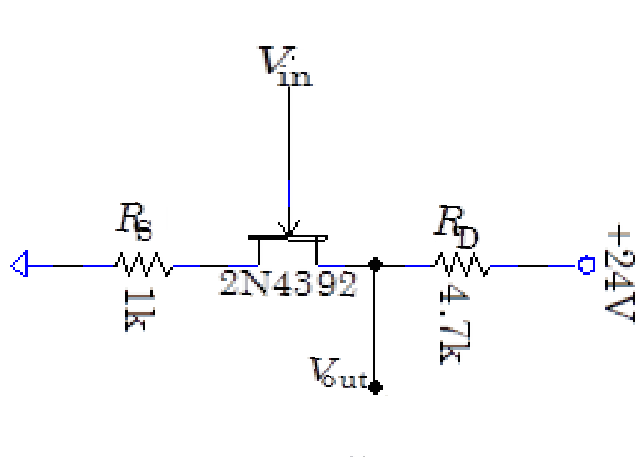
\includegraphics[width=0.4\textwidth]{figure/q1setup}
\caption{Schematic of an amplifier.}
\label{q1setup}
 \end{figure}
\par Without the signal applied, we measured the voltages across the respective terminals of the JFET and current through the drain and source to get a $V_{GS}$ value of 1.60V$\pm$0.592 mV,  $V_{DS}$ of 11.42V $\pm$ 5.3704mV,  $I_{DS}$ of  $0.0149\pm 2.188\times 10^{-6}$mA. The theoretical gain is computed as below, by assuming that the assumption that the trans-conductance is high: 
\begin{equation}
G = - \frac{R_D}{R_s+r_s}\approx -\frac{R_D}{R_s}
\end{equation}
and obtain a predicted gain of -4.7.%Our experimental gain was computed from the $-\frac{V_{out}}{V_{in}}$ ratio and we obtained a value of -5. 
\par We drove the amplifier with a 10kHz , $1V_{pp}$ signal sine wave and record the $V_out$. The V$_{out}$ is measured at 200mV when we input a signal of 1.00V. So we compute the gain by taking the ratio of the voltage output and input:
\begin{equation}
\text{Gain} = -\frac{V_{out}}{V_{in}}=\frac{1.00V}{200mV}=-5
\label{gain_experimental}
\end{equation}
The experimental value is within $\approx 10\%$ of the theoretical predicted value.
\par As we tune the waveform generator, the maximum undistorted output amplitude is found to be 4.30V, and above that we can clearly see that the bottom part of the output signal is flat, as shown in Fig.\ref{q1trace} 
 \begin{figure}[h!]
 \centering
 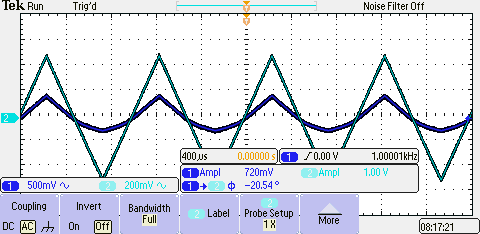
\includegraphics[width=0.4\textwidth]{figure/q1trace}
\caption{Scope trace for the distorted output signal. Channel 1 shows the output signal and Channel 2 shows the original input signal.}
\label{q1trace}
 \end{figure}
\par The fact that the gain is also a function of the $V_{in}$ is what limits the amplitude. The diode in the JFET rectifies the bottom portion of the signal as we have seen in the previous lab. But for a small signal amplitude, the effect is negligible, however for larger amplitude (>4.3V) this functional dependency of the gain results in the distortion.  
\par There is not much change in the output amplitude when the JFET is cooled, the gain remains at around 4, as we have previously found in \ref{gain_experimental}. By substituting our JFET with four other JFETS and examining its cooling behaviour, we found that the gain for each JFET is still around 4 as shown in the $- \frac{V_{out}}{V_{in}}$ calculations below: 
\begin{align*}
Gain_{JFET1}= -\frac{40.8V}{9.80V}=-4.16
\\ Gain_{JFET2}=  -\frac{40.0V}{9.80V}=-4.08
\\ Gain_{JFET3}=  -\frac{40.8V}{9.90V}=-4.12
\\ Gain_{JFET4}=  -\frac{40.8V}{9.80V}=-4.16
\end{align*}
\section*{5.2}
To improve the gain in the Fig.\ref{q1setup} setup, we increased the $R_D$ by a factor of ten. This decreases the $V_{DS}$ substantially to 0.023V$\pm$ 0.0028mV. The gain is much higher than in 5.1 :
\begin{equation}
\text{Gain} = -\frac{990mV}{16mV}= -61.9
\label{gain}
\end{equation}
The higher resistance results in a higher potential drop across  $R_D$, so that no  matter how big the gain is, the $V_{out}$ is still very small. This is evident from the low value of $V_{DS}$, since the voltage drop can occur across  $R_D$ and across the source and drain of the JFET. 
\section*{5.3}
Again, we want to increase the gain: this time by decreasing the $R_s$ in the denominator of Eq.\ref{common_mode_gain}, which describes the common mode gain:
\begin{equation}
Gain = \frac{R_D}{2R_1+R_s+r_s}
\label{common_mode_gain}
\end{equation}
\par In this new setup, the gain is now  -6.43 \footnote{$\frac{-2.96V}{460mV}=-6.43$}.The maximum undistorted output amplitude is1.80$V_{pp}$, beyond this, the scope pattern flattens.
\par Cooling the JFET increases the $V_{out}$, therefore also increases the gain for the same input voltage. We tried these for four other JFETs as summarized in Table.\ref{gain_table}. The fractional variation in the gain is larger for this circuit than the Fig.\ref{q1setup} setup is a result of the 500$\Omega$ source resistor. Since the  impedance of the JFET is comparable to the 500$\Omega$ resistor, the JFET exhibits a stronger temperature dependence. This is not ideal for building electronic circuits and so increasing the gain is not as simple as simply increasing the source resistance.
\begin{table}[h!]
\centering
    \begin{tabular}{l|l|l}
    JFET & Before & After \\ \hline
    1    & -6.04  & -6.39 \\ \hline
    2    & -7.43  & -7.48 \\  \hline
    3    & -3.74  & -6.26 \\ \hline
    4    & -4.17  & -4.00 \\
    \end{tabular}
  \caption{Computed gain values for four JFETs, before and after cooling.The percentage increase of most JFETs were within 10\% (With the exception of JFET 3 which seems to be an  outlier.)}
\label{gain_table}\end{table}
\section*{5.4}
\par We increase the gain by bypassing the source resistor with the addition of a 1$\mu$F capacitor across the source resistor.  By feeding in a 10kHz, 1V$_{pp}$, sine wave, the gain we experimentally computed was -30.9. We compute the source resistance as the total impedance of the RC combination as : 
\begin{equation}
Z = \frac{1}{\sqrt{(\frac{1}{R})^2+(wc)^2}}
\end{equation} Plugging in w =2$\pi$(10kHz) and the nominal value for R, we get Z = 15.9$\Omega$. Then we substitute this relation as source resistor ($R_S$) into the gain equation by :
\begin{equation}
G\approx \frac{-R_D}{R_S}=-\frac{4.7k\Omega}{15.9\Omega}
\label{gain2}
\end{equation}
which yields a gain of around 296. We scan through different frequency and measure the $V_{in}, V_{out} $ for computing the gain. We find that generally as the frequency increase, the gain also increases.
\par This bypassing setup still yields a temperature-dependent circuit. Cooling the JFET caused a 18.11\% increase in the output voltage, and thereby the same percent change in the gain. Compared with the circuit in 5.3 this is even more temperature-dependent. This strong temperature dependence arise from the fact that temperature decrease results in a lower $r_s$. This results in a larger G, since G is inversely proportional to $r_s$ as shown in Eq.\ref{gain2}. %The capacitor increases the gain because the parallel resistance-capacitor subcircuit has a lower impedance than just the 1k$\Omega$ alone, resulting in a larger output voltage, thereby increasing the gain.
\section*{5.5}
 We built the differential amplifier as shown in \ref{q5setup} by connecting the two 100k$\Omega$ and 10k$\Omega$ resistors to ground. Driving the $V_+$, with 1kHz, 0.1$V_{pp}$ sine wave, we get a signal amplitude of 3.00$\pm3.64\times10^{-4}$ V. Connecting the scope to the $V_{invout}$ terminal, we get approximately the same amplitude. The phase measurement is 140.7$^{\circ}$  and -54$^{\circ}$  respectively.
 \par Then we drive the $V_-$ using the same signal and we again obtain a signal amplitude of 3.00$\pm3.64\times10^{-4}$ V. Connecting the scope to the $V_{invout}$ terminal, we get approximately the same amplitude. The phase measurement is -82.50$^{\circ}$ and 70.00$^{\circ}$  respectively. Such behavior is expected because the two sides of the differential amplifier is supposed to exhibit symmetrical behavior, so it does not matter whether we drive on $V_{+}$ or $V_{-}$.
 \par Next, we drive both $V_{+}$ or $V_{-}$ with the same 0.1V signal and obtain $V_{out}$ of 1.00V, so the common mode gain is around 10. By putting on a random JFET, the $V_{out}$ is 1.35V. Along with the voltage drop measurement across the $R_{drain}$ measured at 6.23V and another measured at 1.00V, this deviation from the previously measured voltage drop leads us to conclude that the differential amplifier circuit does not work anymore if we connect a pair of unmatched JFET.
 \begin{figure}[h!]
 \centering
 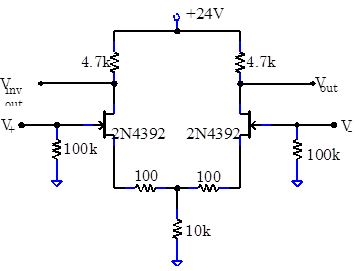
\includegraphics[width=0.5\textwidth]{figure/q5setup}
\caption{Differential amplifier schematic.}
\label{q5setup}
 \end{figure}
 \par Due to the left-right symmetry of the circuit, the resulting voltage is approximately the same when driven from $V_+$ and $V_-$, and when measured from $V_{invout}$ and $V_{out}$. There is a $\approx$180$^{\circ}$  phase shift between the input and output signal.
  \section*{5.6}
By driving a 100mV$_{pp}$ input signal on both terminal we obtain the results summarized in Table.\ref{table2}.
\begin{table}
    \begin{tabular}{l|l|l}
    V$_{out}$/V Amplitude (mV)  & 720   & 820    \\ \hline
    V$_{out}$/V Phase($^{\circ}$)  & 140.7 & -82.50 \\ \hline
    V$_{invout}$/V Amplitude(mV)  & 710   & 860    \\ \hline
    V$_{invout}$/V Phase($^{\circ}$) & -54   & 70     \\
	\end{tabular}
    \caption{Amplitude and phase measurements from V$_{invout}$ and V$_{out}$.}
    \label{table2}
\end{table}
\section*{5.7}
We feed a 1kHz, 0.1V$_{pp}$, triangular wave and varied the output amplitude with the potentiometer on the attentuator, as shown in Fig.\ref{q7setup}.
 \begin{figure}[h!]
 \centering
 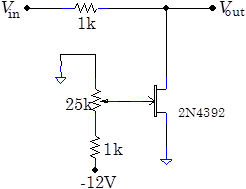
\includegraphics[width=0.4\textwidth]{figure/q7setup}
\caption{JFET Attenuator setup.}
\label{q7setup}
 \end{figure}
 We find that the signal becomes distorted beyond a certain amplitude. The circuit is linear because it still retains the triangular form, however it becomes nonlinear as we go to amplitudes beyond 300mV. This is probably due to the JFET which has a linear (Ohmic) region at lower voltages \footnote{Towards the left hand side of the JFET characteristic curve which plots $I_D$ and $V_{DS}$.} and exhibits nonlinear behaviors at higher voltages.
  \begin{figure}[h!]
 \centering
 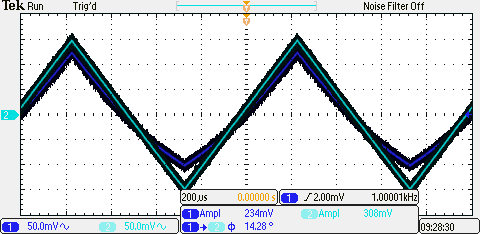
\includegraphics[width=0.5\textwidth]{figure/q7trace}
\caption{Channel 1 shows the distorted signal for an amplitude slightly beyond 300mV. This can be compared with the Channel 2 original signal in cyan.}
\label{q7trace}
 \end{figure}
  \section*{5.8}
  In order to linearize the attentuator shown in Fig.\ref{q7setup}, we added two 100k$\Omega$ resistors.  We set the potentiometer so that we achieve the greatest attenuation on the input signal.   
  \begin{figure}[h!]
 \centering
 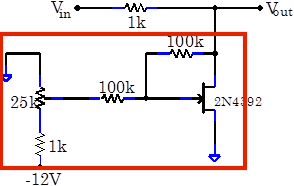
\includegraphics[width=0.5\textwidth]{figure/q8setup}
\caption{JFET Attenuator schematic.}
\label{q8setup}
 \end{figure}
Treating the whole red boxed region as $R_2$ in Fig.\ref{q8setup}, we use the voltage divider equation to find the drain source resistance: 
\begin{align*}
V_{out} = \frac{R_2}{R_1+R_2}V_{in}
\\230mV = \frac{R_2}{1000\Omega+R_2}(318mV)
\label{voltage_divider}
\end{align*}
Solving for $R_2$ yields 2613$\Omega$, this is the lowest possible JFET drain-source resistance corresponding to this setting.

\par The largest input signal that can pass relatively distorted is 500mV. After setting the potentiometer to this maximum attainable attentuation, we measured the gate source voltage as 3.1263V$\pm$0.8mV and the drain source voltage as 30.259mV$\pm$0.008mV. The $V_{in}$ is measured at 3.18mV$\pm$0.04mV and $V_{out}$ is measured at 230mV$\pm$0.03mV.
  \begin{figure}[h!]
 \centering
 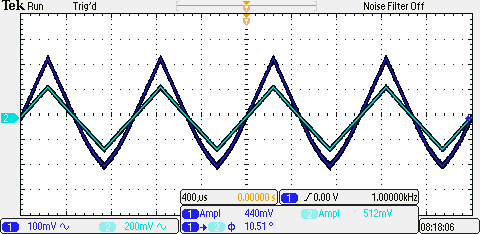
\includegraphics[width=0.5\textwidth]{figure/q8trace}
\caption{The Channel 1 trace shows that beyond the limit of 500mV, the signal can become distorted.}
\label{q8trace}
 \end{figure}
%%%%%%%%%%%TILLL HERE%%%%%%%%%%%%
 \section*{5.9}
We built the JFET Modulator circuit as shown in Fig. \ref{q9setup} and feding in a 1V$_{pp}$input carrier wave of 1MHz, by adding  a 1.0$\mu$F capacitor to the JFET attenuator circuit. Using another function generator to drive the a 1kHz, 1V$_{pp}$ sine wave on the potentiometer gate signal, we find that the input carrier wave (1MHz) is modulated by the 1kHz wave. The modulated output signal is shown in Fig.\ref{q9trace}.   
  \begin{figure}[h!]
 \centering
 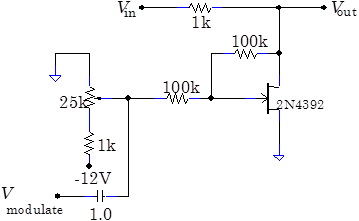
\includegraphics[width=0.5\textwidth]{figure/q9setup}
\caption{JFET Modulator schematic.}
\label{q9setup}
 \end{figure}
 \begin{figure}[h!]
 \centering
 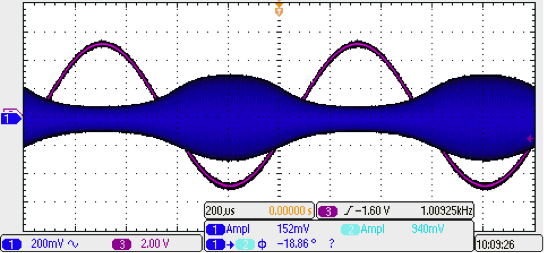
\includegraphics[width=0.5\textwidth]{figure/q9trace}
\caption{Scope traces for the AM signal. Channel 1 shows the modulated $V_{out}$, whose amplitude has a lower resulting amplitude than the 1kHz signal in Channel 3.}
\label{q9trace}
 \end{figure}
  \section*{5.10}
	We tune the AM radio to a quiet channel in the AM band at around 540kHz. The wire is connected to the $V_{out}$ and acts as an AM transmitter for the output signal. We tune the frequency of the modulating signal from the wave generator and then heard the audio signal when the modulating frequency is adjusted to 552kHz. This modulating frequency is very close to the bands that our AM radio is tuned to detect. \footnote{We also found that the signal sounds a lot cleaner if we coiled the transmitting wire around the antenna of the AM radio receiver.} 
\section*{5.11}
Due to the left-right symmetry on both sides of the differential amplifier, \footnote{In theory, the same JFET,$R_D$ and $R_S$.} both JFETs responds the same way to the . As the differential amplifier is built from a matched pair of transistors on both sides. Therefore it is value to assume that the transistors are approximately identical, having a common mode drive. The common mode gain is computed by: 
\begin{align*}
\text{Gain}=	\frac{R_D}{2 Z_{out}+R_s+r_s}  = \frac{R_D}{2 Z_{out}+R_s+1/g}
\end{align*}
where g is the JFET's trans-conductance \footnote{ This should be simmilar for both JFETs}
\par The differential gains for the differential amplifier is computed as : 
	\begin{align*}
	\text{Gain}= \frac{R_D}{R_S+r_s} = \frac{R_D}{R_S+1/g}
	\end{align*}
   \section*{5.12}
  We fed in +24V input on both sides of the surprise circuit as shown in Fig.\ref{q12setup}. 
   \begin{figure}[h!]
 \centering
 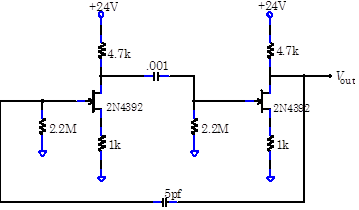
\includegraphics[width=0.4\textwidth]{figure/q12setup}
\caption{Surprise circuit setup.}
\label{q12setup}
 \end{figure}
  The circuit acts like a periodic timer, outputting a square wave with period of 1200$\mu$s. This happens because the voltage through the 0.001$\mu$F capacitor pinches off. Then, after some time period, the capacitor charges up and the 5pF capacitor also pinches off. Since there is quite a difference between the capacitance of the two capacitor, this explains the pattern shown in Fig.\ref{q12trace} as the signal is comprised of a prolonged flattened region followed by a short dip (which is actually a much shorter flattened region).   %(MUST EXPLAIN WHY??)
 \begin{figure}[h!]
 \centering
 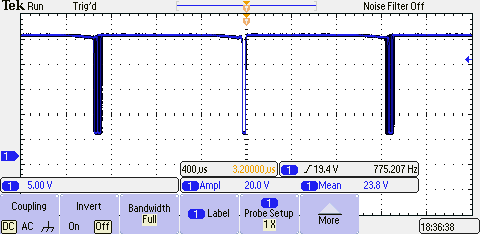
\includegraphics[width=0.4\textwidth]{figure/q12trace}
\caption{Channel 2 shows the original DC signal, which is just noise.}
\label{q12trace}
 \end{figure}
\section*{5.13}
\par We designed and built a unity gain phase splitter as shown in Fig.\ref{q12setup}. We connected a 12V power supply to the $V_{out +}$ terminal and fed in a 1V$_{pp}$, 1kHz sine wave. 
   \begin{figure}[h!]
 \centering
 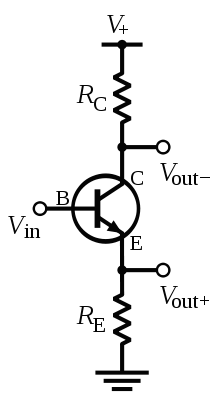
\includegraphics[width=0.15\textwidth]{figure/q13setup}
\caption{Phase Splitter Design. We set both the $R_E$ and the $R_C$ equal to 10k$\Omega$ in order to split the two signals into equal magnitude and opposite phase.}
\label{q12setup}
 \end{figure}
\par As intended, the circuit splits the input signal into two signal (as shown on Channel 1 and 3 of Fig.\ref{q13trace}). We observe that these two signals are almost 180$^{\circ}$ out of phase with each other. The phase splitting resulted in a $V_{out -}$ output signal amplitude that is a few orders of magnitude less than$V_{out +}$. This is due to the fact that the roughly-half-a-period phase shift causes the superposition of the input signal and the $V_{out - }$ to almost zero (24.8mV), whereas the superposition of the input and  the $V_{out + }$ adds up to a larger amplitude of 0.70V.  
    \begin{figure}[h!]
 \centering
 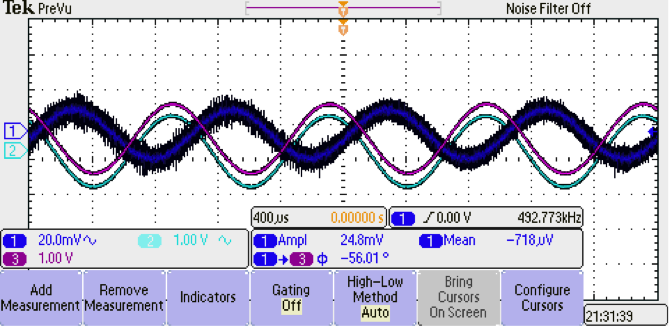
\includegraphics[width=0.5\textwidth]{figure/q13trace}
\caption{Channel 1 shows the measure of $V_{out - }$ ; Channel 2 shows the original input signal; Channel 3 shows the $V_{out +}$}
\label{q13trace}
 \end{figure}
\section*{5.14}
We built a temperature, and JFET-independent high gain amplifier as shown in Fig.\ref{q14setup}. We substituted a $R_1$resistor of 520k$\Omega$ and a  $R_2$1k$\Omega$ resistor for the circuit. The gain was computed from the input and output voltage ratio as $\frac{9.12V}{228mV}=40$. Unlike the previous circuits that we built, the circuit was not perturbed as we cooled it and maintained approximately the same gain .
\begin{figure}[h!]
 \centering
 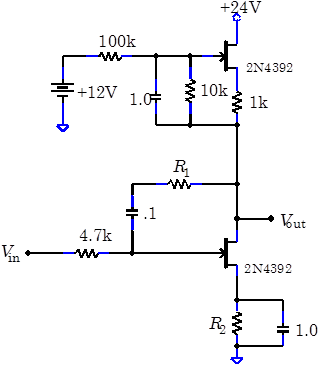
\includegraphics[width=0.4\textwidth]{figure/q14setup}
\caption{High Gain Amplifier Circuit}
\label{q14setup}
\end{figure}
\par Using an unmatched  JFET, the gain was reduced to 14 ($\frac{1.44V}{0.10V}$). Using a new unmatched pair of JFET the gain decreased to a even lower value of 2. The distinction between the former and latter case is that the $R_1$ and $R_2$ we used was not chosen to be the right ones for obtaining a gain of 40 for the new JFETs. However this should not have mattered because the feedback designed in this high gain amplifier should have made the circuit independent of JFET characteristics. Since the JFET is operating at the linear regime, the gain of the circuit can be simply calculated as a voltage divider:
\begin{equation}
\text{Gain} = -\frac{R_D}{R_s+r_s} = -\frac{R_D}{Z_{out}+1/g}
\end{equation}
where the $Z_{out}$ is the finite stiffness of the current source and g is the transconductance of the JFET, following the same line of reasoning in our  5.11 differential gain derivation.
\section*{5.15}
\begin{enumerate}
\item The $R_1$ and the associated subcircuit containing 0.1$\mu$F capacitor sets the gain through feedback since it has direct control over $V_{out}$, which is used to compute the gain.
\item The entire top half of the circuit acts as a current source to increase the gain. This current source is has high current gain and is self-biased.  It serves as a stiff current source to the lower half of the circuit.
\item The $R_2$ resistor and $1\mu$F capacitor increases the open-loop gain by providing an AC bypass capacitor.
\item  The lower part of circuit JFET operates in a linearize regime, therefore we can treat the JFET's impedance as a resistor. The $R_2$ and $1\mu$F capacitor
\item The 12V voltage supply assures that the drain source voltage across both JFETs is approximately 12V. This 12V voltage supply is independent of the JFET characteristic. 
\item There is an oscillation of current between 1.0$\mu$F capacitor in the top half of the circuit until it equilibriates. This provides a bypass for AC signals and increases the stiffness of the current source.
%and the generates the AC current. So makes AC 
\end{enumerate} 
 \section*{Conclusion}
In this lab, we investigated the various applications of JFETs in electronic circuits. We build and design an amplifier, attenuator, modulator, timer and a phase splitter using JFETs along with different combination of resistors and capacitors on the source, gate, and drain terminals. We further explore the characteristics of JFETs through its effects on the circuits such as the temperature-dependent gain in 5.3 and the importance of the ``matched" JFETs as seen in 5.5. Finally, we investigate an operational amplifier circuit contructed from JFETs.
\section*{Acknowledgments}
\begin{footnotesize}
The author would like to acknowledge support from the GSI in this lab in addressing our questions about the lab and with the handling of liquid nitrogen. I would also like to thank my partner, Leah Tom, for helpful discussion and collaboration that helped this work. We also appreciate Sissi Wang for providing us with guidance on question 5.14.
\end{footnotesize}
  \section*{References}
 \begin{footnotesize}
 \begin{itemize}
 \item Horowitz, Paul, and Winfield Hill. \textit{The Art of Electronics}. Cambridge: Cambridge UP, 1989. Print.
 \item ``Lab 5 - JFET Circuits II. " \textit{Donald A. Glaser Advanced Lab.} Regents of the University of California, n.d. Web. 01 Feb. 2015.
 \item \textit{Phase Splitter}. Digital image. \textit{Wikipedia}. Wikimedia Foundation, n.d. Web. 03 Mar. 2015.
 \end{itemize} 
  \end{footnotesize}

\end{document}
